\subsubsection{Caso d’uso UC8.2.6: Modifica domanda a ordinamento di stringhe}
	\label{UC8.2.6}
	\begin{figure}[ht]
		\centering
		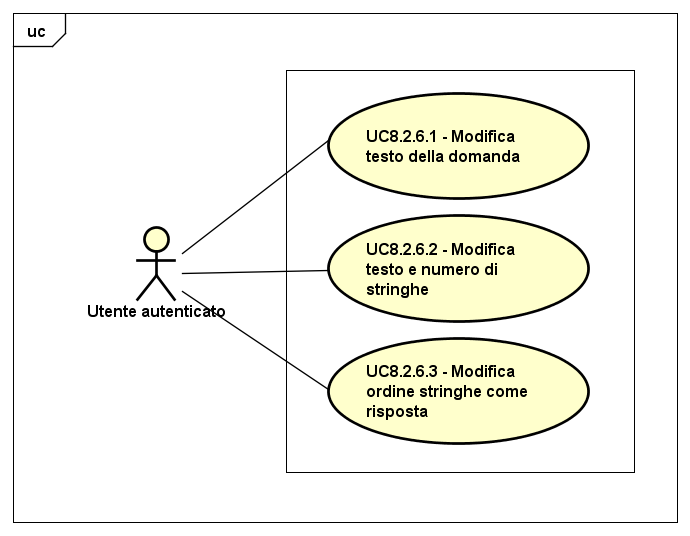
\includegraphics[scale=0.45,keepaspectratio]{UML/UC8_2_6.png}
		\caption{UC8.2.6: Modifica domanda a ordinamento di stringhe}
	\end{figure}
	\FloatBarrier
\begin{itemize}
	\item\textbf{Attori}: utente autenticato, utente autenticato pro;
	\item\textbf{Descrizione}: l'attore può utilizzare la procedura guidata per la modifica di una domanda a ordinamento di stringhe;
	\item\textbf{Precondizione}: il sistema ha ricevuto dall'attore la domanda da modificare; 
	\item \textbf{Postcondizione}: l'attore ha modificato una domanda a ordinamento di stringhe;
	\item\textbf{Scenario principale}:
		\begin{itemize}
			\item L'attore può modificare il testo della domanda (UC8.2.6.1);
			\item L'attore può modificare il testo e il numero delle stringhe che compongono la sequenza della domanda (UC8.2.6.2);
			\item L'attore può modificare l'ordine corretto delle stringhe che costituiscono la risposta (UC8.2.6.3).
		\end{itemize}
\end{itemize}

\subsubsection{Caso d'uso UC8.2.6.1: Modifica testo della domanda}
\begin{itemize}
	\item \textbf{Attori}: utente autenticato, utente autenticato pro;
	\item \textbf{Descrizione}: l'attore può modificare il testo della domanda;
	\item \textbf{Precondizione}:  il sistema mostra la funzionalità di modifica di una domanda a ordinamento di stringhe; 
	\item \textbf{Postcondizione}: l'attore ha modificato il testo della domanda;
	\item \textbf{Scenario principale}: l'attore modifica il testo della domanda.
\end{itemize}

\subsubsection{Caso d'uso UC8.2.6.2: Modifica testo e numero di stringhe}
\begin{itemize}
	\item \textbf{Attori}: utente autenticato, utente autenticato pro;
	\item \textbf{Descrizione}: l'attore può modificare il testo e il numero di stringhe che costituiscono la risposta alla domanda;
	\item \textbf{Precondizione}:  il sistema mostra la funzionalità di modifica di una domanda a ordinamento di stringhe;
	\item \textbf{Postcondizione}: l'attore ha modificato il testo e il numero delle stringhe che costituiscono la risposta alla domanda;
	\item \textbf{Scenario principale}: l'attore modifica il testo e il numero delle stringhe che costituiscono la risposta alla domanda.
\end{itemize}

\subsubsection{Caso d'uso UC8.2.6.3: Modifica ordine stringhe come risposta}
\begin{itemize}
	\item \textbf{Attori}: utente autenticato, utente autenticato pro;
	\item \textbf{Descrizione}: l'attore può modificare l'ordine corretto delle stringhe che rappresenta la soluzione della domanda;
	\item \textbf{Precondizione}:  il sistema mostra la funzionalità di modifica di una domanda a ordinamento di stringhe; 
	\item \textbf{Postcondizione}: l'attore ha modificato l'ordine delle stringhe che costituiscono la risposta alla domanda;
	\item \textbf{Scenario principale}: l'attore modifica l'ordine delle stringhe che costituiscono la risposta alla domanda.
\end{itemize}
